\Section{Typography and direction of reading}{Jarno Smets}

\lettrine{A}{tlan's} writing system is a natural application of our philosophy: start with elementary parts, and every complexity will be a mere combination of those parts. Our glyphs (as we shall call them) each denote one syllable. They always do so; they always will stand for the {\it same} syllable. Unlike English: in the words \lq\lq tone\rq\rq and  \lq\lq to\rq\rq, the \lq\lq to\rq\rq is pronounced respectively [t\textturnm] and [t\textbaro]. 

That is the rationale behind our writing system; let us dive into the details. As told, Atlan has a set of basic lines. They are:

\begin{center}

\begin{tabular}{c|c| m{1cm} |c}
\hline
\multicolumn{2}{c}{Consonants} & \multicolumn{2}{c}{Vowels} \\ 
\hline
{\bf Line} & {\bf In I.P.A.} & {\bf Line} & {\bf In I.P.A.} \\
\DeclareStroke{\CenterVertical} & /t/ & \Atlanu & /u/ \\  
\hline
\DeclareStroke{\CenterHorizontal} & /k/ &  \Atlani & /i/ \\ 
\DeclareStroke{\BigNW} & /j/ & \Atlana & /a/ \\ 
\DeclareStroke{\BigSW} & /s/ & \Atlano & /o/ \\ 
\DeclareStroke{\BigSE} & /f/ & \Atlane & /e/ \\
\DeclareStroke{\BigNE} & /l\~ r/ & & \\
\DeclareStroke{\Dot{Center}} & /p/ & &\\
\DeclareStroke{\MediumCircle{Center}} & <nil\footnotemark> & & \\
\end{tabular}

\end{center}
{\it Figure 1: The basic lines of Atlan's writing system.} \footnotetext{When you see this hollow cirlce, the other line is combined with nothing. Don't panic if you don't yet understand this; it will be explained shortly.}

These lines all represent a single vowel ({\it V}), or a single consonant ({\it C}). We can combine them to make syllables. By combining two consonant lines, you get a CVC-syllable, such as {\it loj}, {\it pas} or {\it mup}. You can also make a VC-syllable, such as {\it mu}, {\it po}, or {\it ji}. The vowels don't have separate lines in a CVC or VC-syllable; instead, the vowel is determined by the position of the two consonant-lines. We will go deeper into that below. First, we give the rules for the order of the consonants and vowels: what determines whether two lines make e.g. {\it poj} or {\it jop}, {\it mu} or {\it um}? 

This order is determined by the manner in which the lines combine. There is always a \lq\lq bigger \rq\rq line, and a smaller one. These lines fit inside an imaginary box. The position of the smaller line relative to the bigger line, determines the order of consonants. A general rule of thumb is best given with the help of a box:

\begin{center}

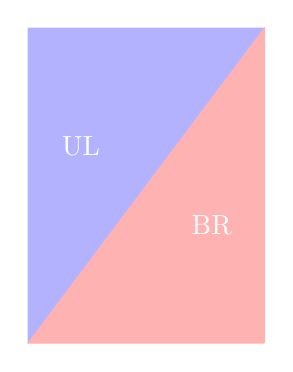
\begin{tikzpicture}
\draw[blue!30, fill= blue!30] (0,0) -- (3,4) -- (0,4) -- (0,0);
\draw[red!30,fill =red!30] (3,0) -- (3,4) -- (0,0) -- (3,0);
\node(A) at (0.67,2.5){\color{white} UL};
\node(B) at (2.33,1.5){\color{white} BR};
\end{tikzpicture}

{\it \footnotesize Figure 2: Box for determining consonant order.}
\end{center}

\noindent If the smaller line is in the upper-left triangle (UL), it the consonant it designates comes first. If it is in the bottom-right one, it comes second. For the rest of the explanation, it is advised to keep this box in the back of your head. An example:

\def\restorecorps{\renewcommand{\corpsgrootte}{20pt}}
\begin{wrapfigure}[7]{l}{0.4\textwidth}
\renewcommand{\corpsgrootte}{100pt}
\kus
\restorecorps
\end{wrapfigure}
\vspace{0.2cm}

As you see here, the smaller line is found on top. Hence, it is placed inside the upper-left triangle. The consonant for which the smaller horizontal line stands (the {\it k}), comes before the other consonant, the {\it s}.

\phantom{}

\begin{center}
\definecolor{melon}{RGB}{255,179,179}
\definecolor{caian}{RGB}{204,255,247}
\definecolor{lavender}{RGB}{242,179,255}
\definecolor{jasmine}{RGB}{255,212,128}
\definecolor{lemon}{RGB}{255,247,204}
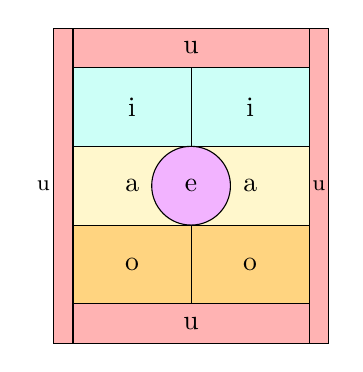
\begin{tikzpicture}
\draw[black] (0,0) rectangle (3,4);
\draw[fill = melon] (0,4) rectangle (3,3.5);
\draw[fill = melon] (0,0.5) rectangle (3,0);
\draw[fill = melon] (-0.25, 0) rectangle (0,4);
\draw[fill = melon] (3.25, 0) rectangle (3,4);
\draw[fill = caian] (1.5,2.5) rectangle (0,3.5);
\draw[fill = caian] (1.5,2.5) rectangle (3,3.5);
\draw[fill = jasmine] (1.5,1.5) rectangle (0,0.5);
\draw[fill = jasmine] (1.5,1.5) rectangle (3,0.5);
\draw[fill = lemon] (1.5,1.5) rectangle (0,2.5);
\draw[fill = lemon] (1.5,1.5) rectangle (3,2.5);
\draw[fill = lavender] (1.5,2) circle (0.5);
\node at (1.5,3.75){u};
\node at (0.75,3){i};
\node at (2.25,3){i};
\node at (0.75,2){a};
\node at (2.25,2){a};
\node at (0.75,1){o};
\node at (2.25,1){o};
\node at (1.5,0.25){u};
\node at (1.5,2){e};
\node at (-0.375, 2){\footnotesize u};
\node at (3.125, 2){\footnotesize u};
\end{tikzpicture}
\end{center}

{\footnotesize \it Figure 3: Location of the smaller line in relation to the vowel.}
\vspace{0.5cm}

The vowel is...
\begin{itemize}
\setlength{\itemsep}{0.25em}
\item {\it u\ }if the smaller line is found at the edges. The smaller line is in its whole above, under, left or right of the main line. 

\item {\it i\ } if the smaller line is found on the upper-left or upper-right side of the main line. It is usually smaller than the line made for {\it u}, to avoid confusion. 

\item {\it a\ } if the smaller line is found left or right to the middle of the line. 

\item {\it o\ } if the smaller line is found on the bottom-left or bottom-right hand of the main line. Again, this line is smaller than the line for {\it u}. 

\item{\it e\ } if the smaller line is placed in the middle. Or, if the small line intersects with the main line at the middle. In some instances, the small line is then split up by the main line.  
\end{itemize}

Then we have three exceptions to these rules. The first: you can combine two equivalent lines, to make syllables such as {\it pop}, {\it mum}, or {\it lol}. The order of these lines doesn't matter; hence we choose place the smaller line to the upper-left of the main line in such cases. For the vowel {\it u}, there are two small lines, split at the center. For {\it e}, there are either two or three small lines. At least one of those lines crosses through the center of the imaginary box.

The second exception has to do with the k (/k/). That letter had the base line -- , right? It's a horizontal line. Because of that, we have to think of a different box from figure 2 to figure out the consonant-order. The solution is simple: we flip the box. It then looks like this:

\vspace{0.5cm}
\begin{center}
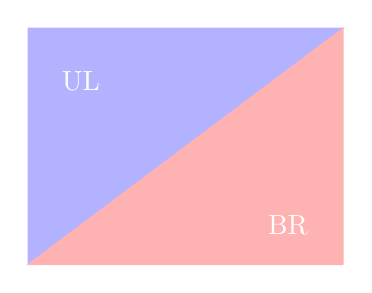
\begin{tikzpicture}

\draw[blue!30, fill= blue!30] (0,0) -- (4,3) -- (0,3) -- (0,0);
\draw[red!30,fill =red!30] (4,0) -- (4,3) -- (0,0) -- (4,0);
\node(A) at (0.67,2.33){\color{white} UL};
\node(B) at (3.3,0.5){\color{white} BR};
	
\end{tikzpicture}
\end{center}

{\footnotesize \it Figure 4: the imaginary consonant-order-box for /k/.}

The third exception: Remember that the {\it p} is represented by the dot $\bullet$\phantom{.}. For clarity, we couldn't combine simply two dots to make a full syllable. Hence, two p-dots combine a bit different from the rest of the lines. The p also can't combine well with the circle (which designated \lq\lq nothing \rq\rq). They combine in the following way:

\begin{center}
\renewcommand{\corpsgrootte}{12pt}
\begin{tabular}{c|c|c|c|c|c|c|}

\multicolumn{2}{l}{Basic line} & u & i & a & o & e\\ 
\hline
\phantom{M} & $\bullet$ & \up & \ip & \ap & \op & \ep \\

$\bullet$ & $\bullet$ & \pup & \pip & \pap & \pop & \pep \\

{$\bullet$} &  & \pu & \Atlanpi & \pa & \po & \pe\\
\end{tabular}
\end{center}
\restorecorps

These were the rules for the script of Atlan. It might sound a bit cryptic, so let's discuss some examples. If you still feel uncertain whether you understand the rules, read through them again. Personal experience tells that, after some time, recognizing letters gets more intuitive. 

\pagebreak

\begin{wrapfigure}[7]{l}{0.4\textwidth}
\renewcommand{\corpsgrootte}{100pt}
\mok
\restorecorps
\end{wrapfigure}

\noindent Let's dissect this letter. This is the letter \lq\lq mok \rq\rq, or ([/mok/]) phonetically. First stept is to discover the main line, which is the long diagonal here. This is the consonant {\it m} (/m/). Then there is a smaller line, found in the bottom-right corner. This is the {\it k} ([/k/]). The horizontal line is in the bottom-right of our imaginary square. Hence, the {\it m} comes before the {\it k} (see also figure one). We got the two consonants, now rests the vowel. Feel free to look back at figure two. The smaller line is found in the bottom-right corner, hence the vowel here is an {\it o} ([/o/]). The full syllable is {\it mok} ([/mok/]). 


\begin{wrapfigure}[7]{r}{0.4\textwidth}
\renewcommand{\corpsgrootte}{100pt}
	\vspace{-1cm}
\jap
\restorecorps
\end{wrapfigure}

\vspace{0.2cm}
Now let's look at another one. See if you can determine the syllable yourself first. The main line is obvious: it's the big curve. This big curve is a {\it j\footnotemark} ([/j/]). The smaller dot is a {\it p} ([/p/]). The dot is found inside the quadrant \lq\lq UL\rq\rq of figure one. Hence, the dot comes first. The dot is found a bit left from the centre of our imaginary box. Hence, the vowel here, is the {\it a} ([/a/]). The full syllable is {\it jap} ([/jap/]). 

\footnotetext{Quick tip: the curve for {\it j} looks alot like the {\it j} itself, doesn't it? Look for more of these similarities in our writing system; they help!}

\begin{wrapfigure}[7]{r}{0.4\textwidth}
\renewcommand{\corpsgrootte}{100pt}
\vspace{-0.5cm}
\lej
\restorecorps
\end{wrapfigure}


Do you feel if you got the hang of it? Let's do a few more. To spice things up a bit, we'll have a syllable with the vowel {\it e}. Remember that this vowel had smaller lines be placed in the centre. Alternatively, the smaller line could intersect the centre, or be split up by it. In this example, the smaller line is split up by the bigger line. The bigger line, the {\it l} ([/l/]) splits up the line for {\it j} ([/j/]). Because it does, the vowel is {\it e} ([/e/]), and the syllable is {\it lej} ([/lej/]). 


\begin{wrapfigure}[7]{l}{0.4\textwidth}
\renewcommand{\corpsgrootte}{100pt}
\vspace{-0.5cm}
\pe
\restorecorps
\end{wrapfigure}

Now the last example. This, we think, is the best-looking glyph in our catalogue. What does it stand for? There aren't two, three, or four separate lines here, as should be. Instead, there is a triangle with a circle inside. What do we do? Well, remember the {\it p} ([/p/]), which was a dot. And remember that \lq\lq nothing \rq\rq also has its line: the circle. There was an exeption for when two p-dots combined, or a p-dot and a circle. The exception was explained a few pages back. If you go there, you encounter the same glyph. This syllable is the {\it pe} ([/pe/]). A tip for remembering these glyphs: if you see a glyph with a triangle and a circle, think of the {\it p}.

We hope the examples have made clear how our writing system works. This concludes the explanation of our writing system for syllables. Upcoming is our writing system for numbers, and for names. Before we get to the next part, a few words of advice for learning the writing system:
\begin{itemize}
	\item On the next pages, a full list of our glyphs is added. They are 490 in number; as many glyphs as we have syllables. Don't be intimidated by the list; instead, use it wisely. Look through the list, and try to grasp the pattern of formation. Read the explanation above, and try to get a feel of how our glyps are formed. Again: after some while, you'll have a stronger intuition. 
	\item Try drawing some of the glyphs. It helps for getting used to the glyps. You don't need a ruler to draw them; just make sure they can be distinguished from each other. 
	\item Any blank space is the \lq\lq nothing \rq\rq we talked about above. You can see the circles appear at the rows of those blank spaces. If the half of an entire row is empty, it means that a combination's reverse is unneccessary. Think of syllables like {\it lol}, {\it nun} or {\it juj}. They are symmetric, so we don't need a full row for them. 
\end{itemize}

Again, on the next page is a table containing all our glyphs. The left two columns contain the base lines, placed in order of combination. If you've forgot which base line stands for which consonant, return to the table at the begin of the chapter. It's a great tool for using as a reference. So come back when you need it.  

%\documentclass[landscape,a5paper]{article}
\usepackage{graphicx}
\usepackage{tikz}                                                                                                                                 
\usepackage{fancyhdr}
\usepackage[tmargin=20pt, bmargin=5pt, rmargin=20pt, margin=5pt]{geometry}
\usepackage{../Atlan}                                                                                                                                
\usepackage{fontspec}                                                                                                                             
\usepackage{longtable}                                                                                                                            
\usepackage[t,lf]{spectral}                                                                                                                       
\usepackage{geometry}                                                                                                                             
\pagestyle{empty}
\begin{document}
\newgeometry{tmargin=50pt, bmargin=5pt}
\fancyhead[R]{3.1. TYPOGRAPHY AND DIRECTION OF READING}
\fancyhead[L]{}

\let\newbullet\bullet
\renewcommand{\bullet}{\raisebox{0.3em}{\newbullet}}
\renewcommand{\corpsgrootte}{15pt}
\begin{longtable}{c c | c c c c c || c c | c c c c c}
	\multicolumn{2}{c}{Base lines} & u & i & a & o & e & \multicolumn{2}{c}{Base lines} & u & i & a & o & e \\
\hline

$\empty$ &  
$\empty$  &
\Atlanu &
\Atlani &
\Atlana &
\Atlano &
\Atlane & 
	&  & & & &  \\

$\empty$  &
\DeclareStroke{\CenterVertical} &
\ut &
\Atlanit &
\at &
\ot &
\et &

\DeclareStroke{\CenterVertical} &
$\empty$ & 
\tu &
\ti &
\ta &
\Atlanto &
\te \\

\DeclareStroke{\CenterVertical} &
\DeclareStroke{\CenterVertical} &
\tut &
\tit &
\tat &
\tot &
\tet &
  & & & & & \\

\DeclareStroke{\CenterVertical} &
\DeclareStroke{\CenterHorizontal} &
\tuk &
\tik &
\tak &
\tok &
\tek &

\DeclareStroke{\CenterHorizontal} &
\DeclareStroke{\CenterVertical} &
\kut &
\kit &
\kat &
\kot &
\ket \\
 
\DeclareStroke{\CenterVertical} &
\DeclareStroke{\RightDiagonal} &
\tun &
\tin &
\Atlantan &
\ton &
\ten &

\DeclareStroke{\RightDiagonal} &
\DeclareStroke{\CenterVertical} &
\nut &
\nit &
\nat &
\Atlannot &
\net  \\



\DeclareStroke{\CenterVertical} &
\DeclareStroke{\LeftDiagonal} &
\tum &
\tim &
\tam &
\tom &
\tem &

\DeclareStroke{\LeftDiagonal} &
\DeclareStroke{\CenterVertical} &
\mut &
\Atlanmit &
\mat &
\mot &
\met \\

\DeclareStroke{\CenterVertical} &
\DeclareStroke{\BigSE} &
\tuf &
\tif &
\taf &
\tof &
\tef &

\DeclareStroke{\BigSE} &
\DeclareStroke{\CenterVertical} &
\fut &
\fit &
\fat &
\fot &
\fet \\

\DeclareStroke{\CenterVertical} &
\DeclareStroke{\BigSW} &
\tus &
\tis &
\tas &
\tos &
\tes &

\DeclareStroke{\BigSW} &
\DeclareStroke{\CenterVertical} &
\sut &
\sit &
\sat &
\sot &
\set \\

\DeclareStroke{\CenterVertical} &
\DeclareStroke{\BigNE} &
\tul &
\til &
\tal &
\tol &
\tel &

\DeclareStroke{\BigNE} &
\DeclareStroke{\CenterVertical} &
\lut &
\lit &
\lat &
\lot &
\Atlanlet \\

\DeclareStroke{\CenterVertical} &
\DeclareStroke{\BigNW} &
\tuj &
\tij &
\taj &
\toj &
\tej &

\DeclareStroke{\BigNW} &
\DeclareStroke{\CenterVertical} &
\jut &
\jit &
\jat &
\Atlanjot &
\jet \\

\DeclareStroke{\CenterVertical} &
$\bullet$ &
\tup &
\tip &
\tap &
\Atlantop &
\tep &

$\bullet$ &
\DeclareStroke{\CenterVertical} &
\Atlanput &
\pit &
\pat &
\pot &
\pet \\


$\empty$ &
\DeclareStroke{\CenterHorizontal} &
\uk &
\ik &
\ak &
\ok &
\ek &

\DeclareStroke{\CenterHorizontal} &
$\empty$ &
\ku &
\ki &
\ka &
\ko &
\ke \\

\DeclareStroke{\CenterHorizontal} &
\DeclareStroke{\CenterHorizontal} &
\kuk &
\kik &
\kak &
\kok &
\kek &
 & & & & & \\


\DeclareStroke{\CenterHorizontal} &
\DeclareStroke{\RightDiagonal} &
\kun &
\kin &
\kan &
\kon &
\ken &

\DeclareStroke{\RightDiagonal} &
\DeclareStroke{\CenterHorizontal} &
\nuk &
\nik &
\nak &
\nok &
\nek \\


\DeclareStroke{\CenterHorizontal} &
\DeclareStroke{\LeftDiagonal} &
\kum &
\kim &
\kam &
\kom &
\kem &

\DeclareStroke{\LeftDiagonal} &
\DeclareStroke{\CenterHorizontal} &
\muk &
\mik &
\mak &
\mok &
\mek \\

\DeclareStroke{\CenterHorizontal} &
\DeclareStroke{\BigSE} &
\kuf &
\kif &
\kaf &
\kof &
\kef &

\DeclareStroke{\BigSE} &
\DeclareStroke{\CenterHorizontal} &
\fuk &
\fik &
\fak &
\fok &
\fek \\

\DeclareStroke{\CenterHorizontal} &
\DeclareStroke{\BigSW} &
\kus &
\kis &
\kas &
\kos &
\kes &

\DeclareStroke{\BigSW} &
\DeclareStroke{\CenterHorizontal} &
\suk &
\sik &
\sak &
\sok &
\sek \\

\DeclareStroke{\CenterHorizontal} &
\DeclareStroke{\BigNE} &
\kul &
\kil &
\kal &
\kol &
\kel &

\DeclareStroke{\BigNE} &
\DeclareStroke{\CenterHorizontal} &
\luk &
\lik &
\lak &
\lok &
\lek \\

\end{longtable}

\pagebreak

\newgeometry{tmargin=20pt, bmargin=30pt}

\begin{longtable}{c c | c c c c c || c c | c c c c c}
\multicolumn{2}{c}{Base lines} & u & i & a & o & e &  \multicolumn{2}{c}{Base lines} & u & i & a & o & e \\
\hline



\DeclareStroke{\CenterHorizontal} &
\DeclareStroke{\BigNW} &
\kuj &
\kij &
\kaj &
\koj &
\kej &

\DeclareStroke{\BigNW} &
\DeclareStroke{\CenterHorizontal} &
\juk &
\jik &
\jak &
\jok &
\jek \\

\DeclareStroke{\CenterHorizontal} &
$\bullet$ &
\kup &
\kip &
\kap &
\kop &
\kep &

$\bullet$ &
\DeclareStroke{\CenterHorizontal} &
\puk &
\pik &
\pak &
\pok &
\pek \\

$\empty$ &
\DeclareStroke{\RightDiagonal} &
\un &
\Atlanin &
\an &
\on &
\en &

\DeclareStroke{\RightDiagonal} &
$\empty$ &
\Atlannu &
\Atlanni &
\na &
\no &
\Atlanne \\

\DeclareStroke{\RightDiagonal} &
\DeclareStroke{\RightDiagonal} &
\nun &
\nin &
\nan &
\non &
\nen \\

\DeclareStroke{\RightDiagonal} &
\DeclareStroke{\LeftDiagonal} &
\num &
\nim &
\nam &
\nom &
\nem &

\DeclareStroke{\LeftDiagonal} &
\DeclareStroke{\RightDiagonal} &
\mun &
\Atlanmin &
\man &
\mon &
\men \\

\DeclareStroke{\RightDiagonal} &
\DeclareStroke{\BigSE} &
\nuf &
\nif &
\naf &
\nof &
\nef &

\DeclareStroke{\BigSE} &
\DeclareStroke{\RightDiagonal} &
\fun &
\fin &
\fan &
\fon &
\fen \\

\DeclareStroke{\RightDiagonal} &
\DeclareStroke{\BigSW} &
\nus &
\nis &
\nas &
\nos &
\nes &

\DeclareStroke{\RightDiagonal} &
\DeclareStroke{\BigSW} &
\sun &
\Atlansin &
\san &
\son &
\sen \\

\DeclareStroke{\RightDiagonal} &
\DeclareStroke{\BigNE} &
\nul &
\Atlannil &
\nal &
\nol &
\nel &

\DeclareStroke{\BigNE} &
\DeclareStroke{\RightDiagonal} &
\lun &
\lin &
\lan &
\lon &
\len \\

\DeclareStroke{\RightDiagonal} &
\DeclareStroke{\BigNW} &
\nuj &
\nij &
\naj &
\noj &
\nej &

\DeclareStroke{\BigNW} &
\DeclareStroke{\RightDiagonal} &
\jun &
\jin &
\jan &
\jon &
\jen \\

\DeclareStroke{\RightDiagonal} &
$\bullet$ &
\nup &
\nip &
\nap &
\nop &
\nep &

$\bullet$ &
\DeclareStroke{\RightDiagonal} &
\pun &
\pin &
\pan &
\pon &
\pen \\

$\empty$ &
\DeclareStroke{\LeftDiagonal} &
\um &
\im &
\am &
\om &
\Atlanem &

\DeclareStroke{\LeftDiagonal} &
$\empty$ &
\Atlanmu &
\mi &
\ma &
\mo &
\me \\

\DeclareStroke{\LeftDiagonal} &
\DeclareStroke{\LeftDiagonal} &
\mum &
\mim &
\mam &
\mom &
\mem &
 & & & & & & \\

\DeclareStroke{\LeftDiagonal} &
\DeclareStroke{\BigSE} &
\muf &
\mif &
\maf &
\mof &
\mef &

\DeclareStroke{\BigSE} &
\DeclareStroke{\LeftDiagonal} &
\fum &
\fim &
\Atlanfam &
\fom &
\fem \\

\DeclareStroke{\LeftDiagonal} &
\DeclareStroke{\BigSW} &
\mus &
\mis &
\mas &
\mos &
\mes &

\DeclareStroke{\BigSW} &
\DeclareStroke{\LeftDiagonal} &
\Atlansum &
\Atlansim &
\sam &
\som &
\sem \\

\DeclareStroke{\LeftDiagonal} &
\DeclareStroke{\BigNE} &
\mul &
\mil &
\mal &
\mol &
\mel &
\DeclareStroke{\BigNE} &
\DeclareStroke{\LeftDiagonal} &
\lum &
\Atlanlim &
\lam &
\lom &
\lem \\

\DeclareStroke{\LeftDiagonal} &
\DeclareStroke{\BigNW} &
\muj &
\mij &
\maj &
\moj &
\mej &

\DeclareStroke{\BigNW} &
\DeclareStroke{\LeftDiagonal} &
\jum &
\jim &
\jam &
\jom &
\jem \\

\DeclareStroke{\LeftDiagonal} &
$\bullet$ &
\mup &
\mip &
\map &
\mop &
\mep &

$\bullet$ &
\DeclareStroke{\LeftDiagonal} &
\pum &
\pim &
\pam &
\pom &
\pem \\

$\empty$ &
\DeclareStroke{\BigSE} &
\uf &
\Atlanif &
\af &
\of &
\ef &

\DeclareStroke{\BigSE} &
$\empty$ &
\fu &
\Atlanfi &
\fa &
\fo &
\fe \\

\DeclareStroke{\BigSE} &
\DeclareStroke{\BigSE} &
\fuf &
\fif &
\faf &
\fof &
\fef &
  & & & & & \\

\end{longtable}

\pagebreak 
\newgeometry{tmargin=50pt, bmargin=5pt}

\fancyhead[R]{3.1. TYPOGRAPHY AND DIRECTION OF READING}
\fancyhead[L]{}

\begin{longtable}{c c | c c c c c || c c | c c c c c}
\multicolumn{2}{c}{Base lines} & u & i & a & o & e & \multicolumn{2}{c}{Base lines} & u & i & a & o & e \\
\hline

\DeclareStroke{\BigSE} &
\DeclareStroke{\BigSW} &
\fus &
\fis &
\fas &
\fos &
\fes &

\DeclareStroke{\BigSW} &
\DeclareStroke{\BigSE} &
\suf &
\sif &
\saf &
\sof &
\sef \\

\DeclareStroke{\BigSE} &
\DeclareStroke{\BigNE} &
\ful &
\fil &
\fal &
\fol &
\fel &

\DeclareStroke{\BigNE} &
\DeclareStroke{\BigSE} &
\luf &
\lif &
\laf &
\lof &
\lef \\

\DeclareStroke{\BigSE} &
\DeclareStroke{\BigNW} &
\fuj &
\fij &
\faj &
\foj &
\fej &

\DeclareStroke{\BigNW} &
\DeclareStroke{\BigSE} &
\juf &
\jif &
\jaf &
\jof &
\jef \\

\DeclareStroke{\BigSE} &
$\bullet$ &
\fup &
\fip &
\fap &
\fop &
\fep &

$\bullet$ &
\DeclareStroke{\BigSE} &
\puf &
\pif &
\paf &
\pof &
\pef \\

$\empty$ &
\DeclareStroke{\BigSW} &
\us &
\is &
\as &
\os &
\es &

\DeclareStroke{\BigSW} &
$\empty$ &
\su &
\sa &
\si &
\so &
\se \\

\DeclareStroke{\BigSW} &
\DeclareStroke{\BigSW} &
\sus &
\sis &
\sas &
\sos &
\ses &
  & & & & & \\

\DeclareStroke{\BigSW} &
\DeclareStroke{\BigNE} &
\sul &
\sil &
\sal &
\sol &
\sel &

\DeclareStroke{\BigNE} &
\DeclareStroke{\BigSW} &
\lus &
\lis &
\las &
\los &
\les \\

\DeclareStroke{\BigSW} &
\DeclareStroke{\BigNW} &
\suj &
\sij &
\saj &
\soj &
\sej &

\DeclareStroke{\BigSW} &
\DeclareStroke{\BigNW} &
\jus &
\jis &
\jas &
\jos &
\jes \\

\DeclareStroke{\BigSW} &
$\bullet$ &
\Atlansup &
\sip &
\sap &
\sop &
\sep &

$\bullet$ &
\DeclareStroke{\BigSW} &
\pus &
\pis &
\pas &
\pos &
\pes \\

$\empty$ &
\DeclareStroke{\BigNE} &
\ul &
\il &
\al &
\ol &
\el &

\DeclareStroke{\BigNE} &
$\empty$ &
\lu &
\li &
\la &
\lo &
\Atlanle \\

\DeclareStroke{\BigNE} &
\DeclareStroke{\BigNE} &
\lul &
\lil &
\lal &
\lol &
\lel &
 & & & & & \\

\DeclareStroke{\BigNE} &
\DeclareStroke{\BigNW} &
\luj &
\lij &
\laj &
\loj &
\lej &

\DeclareStroke{\BigNW} &
\DeclareStroke{\BigNE} &
\jul &
\jil &
\jal &
\jol &
\jel \\

\DeclareStroke{\BigNE} &
$\bullet$ &
\lup &
\lip &
\lap &
\lop &
\lep &

$\bullet$ &
\DeclareStroke{\BigNE} &
\pul &
\pil &
\pal &
\pol &
\pel \\

$\empty$ &
\DeclareStroke{\BigNW} &
\uj &
\Atlanij &
\aj &
\oj &
\ej &

\DeclareStroke{\BigNW} &
$\empty$ &
\ju &
\ji &
\ja &
\jo &
\je \\

\DeclareStroke{\BigNW} &
\DeclareStroke{\BigNW} &
\juj &
\jij &
\jaj &
\joj &
\jej &
 & & & & & \\

\DeclareStroke{\BigNW} &
$\bullet$ & 
\jup &
\jip &
\jap &
\jop &
\jep &

$\bullet$ & 
\DeclareStroke{\BigNW} &
\puj &
\pij &
\paj &
\poj &
\pej \\

$\empty$ &
$\bullet$ &
\up &
\ip &
\ap &
\op &
\ep &

$\bullet$ &
$\empty$ &
\pu &
\Atlanpi &
\pa &
\po &
\pe \\

$\bullet$ &
$\bullet$ &
\pup &
\pip &
\pap &
\pop &
\pep &
 & & & & & \\

\end{longtable}

\end{document}


\pagebreak
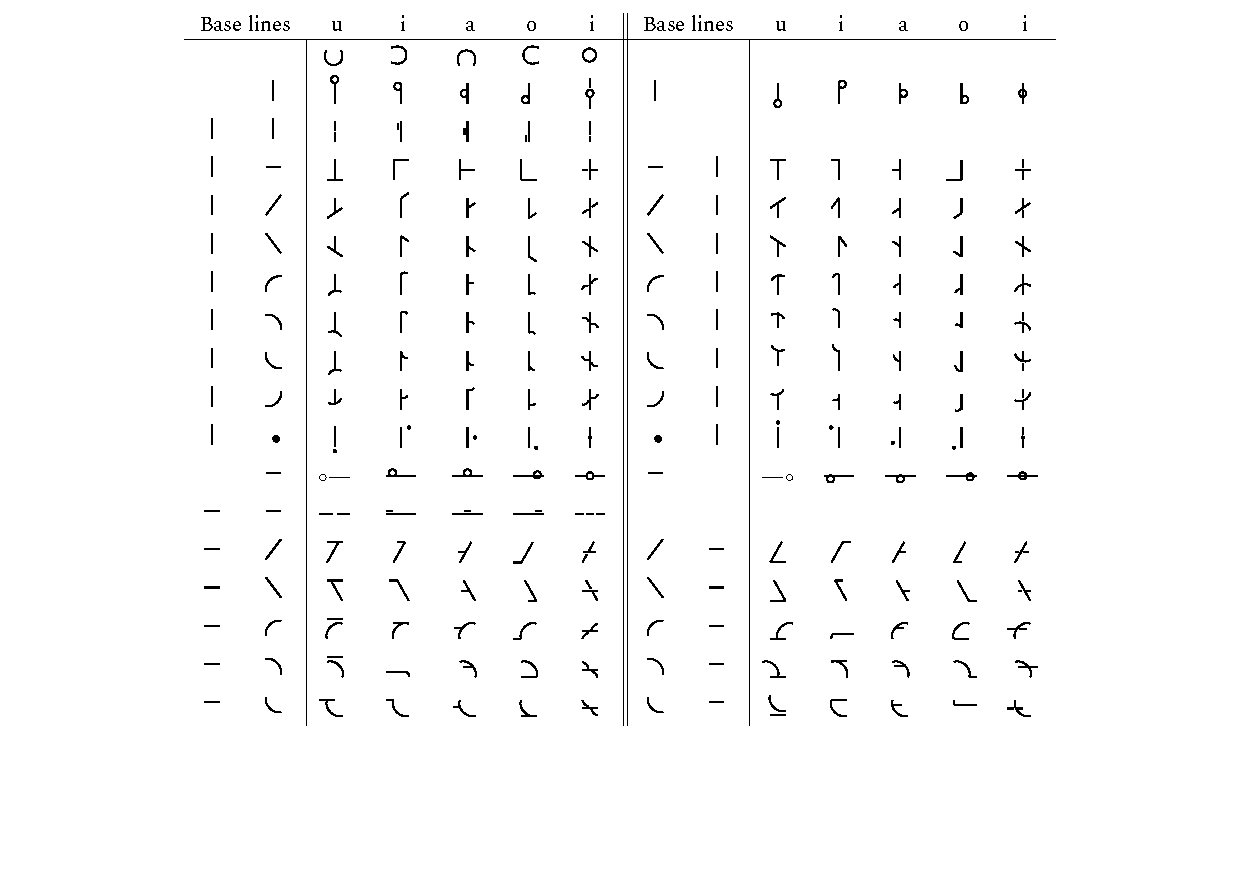
\includepdf[pages=1, pagecommand={}, width = 0.5\pagewidth, angle=90]{./TABEL.pdf}%LE-crop.pdf}
\pagebreak

\includepdf[pages=2, pagecommand={}, width = 0.8\pagewidth, angle=-90]{./TABEL.pdf}%LE-crop.pdf}
\pagebreak

\includepdf[pages=3, pagecommand={}, width = 0.8\pagewidth, angle=90]{./TABEL.pdf}%LE-crop.pdf}

\restoregeometry
\Section{Numerals and Mathematics}{}


\section{Punctuation}
Atlan has minimal punctuation, only having dedicated symbols for a comma and a full stop, and spaces are the same as in any other orthography. A comma is notated as a small half circle which is open at the top: \DeclareStroke{(3.5, -2.5) to [bend left = -50] (4, -2.5)} symbolizing an ‘open’ continuation of the sentence, and the full stop is notated at as a half circle which is open at the bottom: \DeclareStroke{(3.5, -2.5) to [bend left = 50] (4, -2.5)}, symbolizing a closed sentence. 

Other punctuation will be marked by Atlan’s semantic atoms: question sentences start with the interrogative particle E, and so this eliminates the need for a question mark. Exclamative sentences start with the particle O, eliminating the need for an exclamation mark. Other examples would be ‘\&’ being ‘AN’ (‘and’), ‘\%’ being ‘EP.NO’ (‘per hundred’), ‘:’ being ‘I’ (‘relative clause’) etc. 

\section{Transliteration}
Atlan words will be transliterated into the Roman alphabet using the archetype letters U, I, A, O, E, P, T, K, M, N, S, F, L, J. Dots are used in between each syllable, in order to prevent confusion about where syllables are broken up, since this could create ambiguity in meaning. Dots in between two of the same consonants (eg. AK.KA) or vowels (e.g. KA.AK) are pronounced as a glottal stop or shwa, respectively (see chapter 2.2 and 2.3). 

Atlan’s syllables are all (C)V(C). Some loanwords or names, however, might have two or more consonants in a row within the same syllable. In such cases, the individual letter lines that exceed the CVC limit, will stand on their own next to the syllable glyph. The name ‘Stijn’, for example, will then become ‘S.TEJ.N’. 

\section{Numerals}

Atlan also has a numeric system distinct from the familiar arabic-numerals. They look like this:
\pagebreak

\setlength{\columnsep}{10pt}

\begin{multicols}{4}
\small

1  \numbr{1} 

2   \numbr{2}

3   \numbr{3}

4   \numbr{4}

5   \numbr{5}

6   \numbr{6}

7   \numbr{7}

8   \numbr{8}

9   \numbr{9}	

\columnbreak

10   \numbr{10}

20   \numbr{20}

30   \numbr{30}

40   \numbr{40}

50   \numbr{50}

60   \numbr{60}

70   \numbr{70}

80   \numbr{80}

90   \numbr{90}


\columnbreak

100   \numbr{100}

200   \numbr{200}

300   \numbr{300}

400   \numbr{400}

500   \numbr{500}

600   \numbr{600}

700   \numbr{700}

800   \numbr{800}

900   \numbr{900}


\columnbreak

1000   \numbr{1000}

2000   \numbr{2000}

3000   \numbr{3000}

4000   \numbr{4000}

5000   \numbr{5000}

6000   \numbr{6000}

7000   \numbr{7000}

8000   \numbr{8000}

9000   \numbr{9000}




\end{multicols}

The bottom right corner will be the first order of magnitude (below 10), the upper-right corner the second order (tens), the bottom-left corner the third (hundreds) and the top left the fourth (thousands). This way, when reading a single numeral, one would read from left to right and top to bottom, first the thousands, then the hundreds, then the tens and then the below tens, like for example the number 2023 (\numbr{2023}). An empty line is equal to zero (\numbr{0}), and having one of the corners empty but others with a number attached means that that order of magnitude is zero (such as the third order of magnitude in 2023). Decimals can be made by using a comma and adding a numeral behind it: in this case the orders of magnitude are flipped: one behind the comma is a tenth, two is a hundredth, three a thousandth and four a ten thousandth. For example, 2023,2023 would be \numbr{2023}◡\numbr{2023}. 

An added benefit of this numeral system, besides taking less space, is that addition could be more visually intuitive for some numbers: \numbr{1} plus \numbr{3} equals \numbr{4}, \numbr{2} plus \numbr{3} equals \numbr{5}, \numbr{1} plus \numbr{6} equals \numbr{7}. 

Atlan’s numeral system also allows for a duodecimal base notation, with the addition of unique numerals for 10 and 11: 

\vspace{0.2cm}
{\small
10 = \numbr{10}, 120 = (\numbr{120}), 1440 = (\numbr{1440}), 17280 = (\numbr{17280}) 

11 = \numbr{11}, 132 = (\numbr{132}), 1584 = (\numbr{1584}), 19008 = (\numbr{19008}) 
}
\vspace{0.2cm}

The added benefit of a duodecimal system is that certain fractions divisible by 2, 3, 4 and 6 are more straightforward to calculate by heart, whereas 10 can only be divided easily by 2 and 5. Another benefit is that it is more suited for many numerical systems, such as time divided into 60 seconds per 60 minutes per 24 hours, the twelve months and zodiac signs, as well as rotation being divided into 360 degrees.  

\pagebreak
\begin{wrapfigure}{r}{0.4\textwidth}
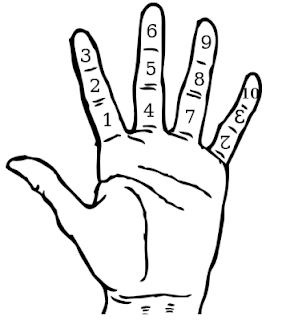
\includegraphics[scale=0.4]{./Images/Hand.jpeg}

	{\it \footnotesize Image taken from West (2015). }
\end{wrapfigure}

The duodecimal system can also be easily counted on a single hand, by using the thumb of the same hand as a pointer to count off the 3 finger segments in the 4 remaining fingers (see figure). Atlans number syllables fit this system as well: 1, 2 and 3 are ´IP´ \ip ´OP´ \op ´UP´ \up, since these all end in P they are grouped together on the first finger. 4, 5 and 6 are ´IK´ \raisebox{-0.5em}{\ik} , ´OK´ \raisebox{-0.5em}{\ok}, ´UK´ \raisebox{-0.5em}{\uk}, following again the same vowel pattern, but with K, grouping them on the second finger. Similarly, 6, 7, and 8 are ´UK´ \uk ´IM´ \im ´OM´ \om, and 9, 10, 11 are ´JI´ \ji ´JO´ \jo ´JU´ \ju. 

Currently, Atlan does not have a standardised system to clarify beforehand whether decimal or duodecimal numerals are used, other than to spot the usage of the numerals \numbr{10} and \numbr{11}. Frankly, current duodecimal systems in Arabic notation don´t have this either, but it could be easily stated verbally beforehand.  

 

\section{Mathematics -- {\small Stijn Janssens}}

Just as with punctuation, mathematical symbols can be approximated by semantic atoms. For example, plus + could be ‘AN’ \an (‘and’), minus - could be ´NE´ \ne (´negative´), divided by : could be ´EP´ \raisebox{-0.5em}{\ep} (´per´), equals = could be ´ME´ \raisebox{-0.3em}{\me} (´equal´). This way, speakers will not be required to learn many new mathematical symbols, but rather the glyphs could function as these, as well as carrying their own pronunciation and meaning. More complicated mathematical symbols or notations might need to be formalized and standardized by mathematicians, which might require more than one syllable. 




\section{Typography}

\begin{center}
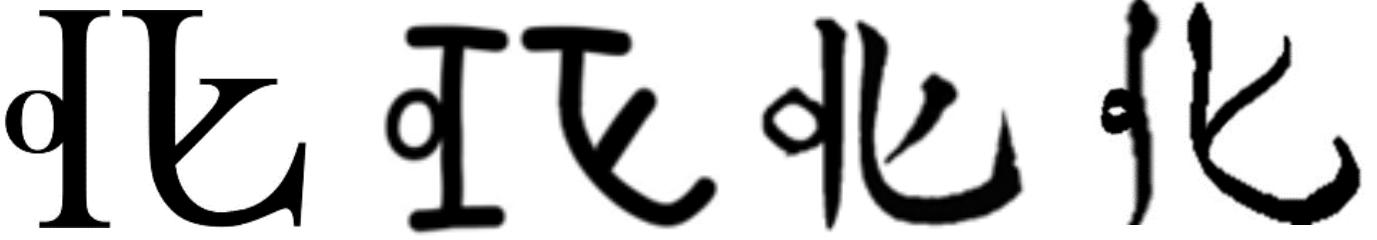
\includegraphics[scale=0.15]{./Images/Atlogos.jpeg}
\end{center}


\noindent Since Atlan’s writing system is comprised of a set of basic lines, a great degree of artistic freedom is possible in creating different fonts and calligraphy styles to write the language. Atlan typography should make sure to remain faithful to the specific orientations of the different lines as to not cause confusion between them. Since any glyph contains a minimal amount of lines, usually two, typographic ornamentation can be added to glyphs without causing much confusion. Here we provide four examples of typographic variations on the word ‘Atlan’: a Times New Roman font, a {\it Comic Sans}-style font, Asian-style calligraphy and Arabic-style calligraphy.


\section{Names, loanwords, and cartouches}

Words that denote certain names, such as personal names, placenames, names for institutions, as well as loanwords denoting certain culture-specific objects or concepts, like certain meals, for example, are incorporated into Atlan as phonetic approximations of these words in their source language. Because every possible syllable in Atlan already has its own designated semantic value, this could cause confusion, if the syllables are interpreted as Atlan words instead of loanwords. For this reason, names and loanwords always follow the following structure: 

\textbf{denoting category (e.g.: person \ej (EJ), place \lu (LU), town \tos (TOS), food \maj \kos (MAJ.KOS)) + NA \na (name) + phonetic approximation} 

Using this formula, ‘Paris’ would become: ‘TOS.NA.PA.LI’ \cartouche{\tos \na \pa \li}, and ‘curry’ would become ‘MAJ.KOS.NA.KA.LI’ \cartouche{\maj \kos \na \ka \li}. If the conversational context makes it explicit enough that the subject matter concerns a loanword, and not a literal Atlan word, the markers denoting category + NA may be omitted for the sake of fluent speech.  

In (formal) typography, a cartouche may be employed to encircle the phonetic approximation in order to enhance intelligibility. Cartouches originate from Ancient Egyptian hieroglyphic orthography, where they were used to encircle the names of pharaohs (see Fig. 1) (Chrisholm, 1911).  

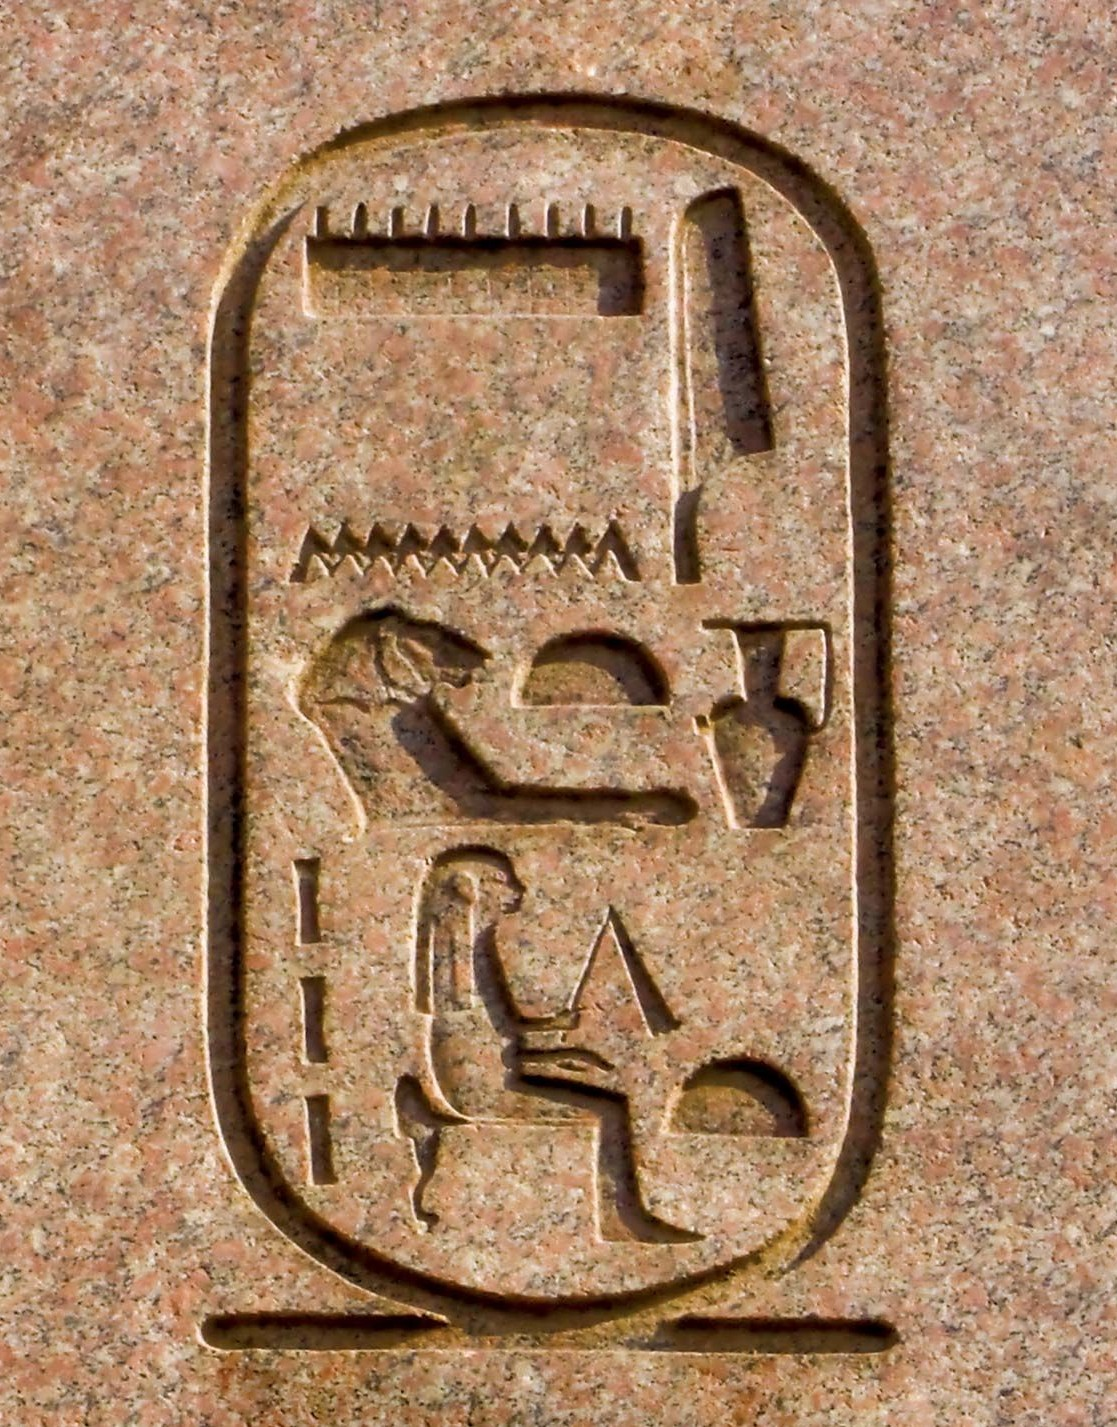
\includegraphics[scale=0.3]{./Images/Cartouche.jpeg}
Fig.1 Cartouche of Hapshepsut, one of the few female pharaohs in Egyptian history. She was often referred to androgynously because of a lack of feminine royal nomenclature (Graves-Brown, 2010). 

 

The cartouche originates from the hieroglyphic ‘shen’, a stylised loop of a rope, which literally means ‘to encircle’, but had come to symbolise eternal protection. Therefore, it was also believed to have apotropaic powers (warding off evil). The word ‘cartouche’ comes from the French word for ‘paper bullet cartridge’, first applied when Napoleon’s soldiers encountered the frequently occurring glyph and noticed its resemblance to such cartridges (White, 2002). Interestingly, cartouches played an important role in deciphering Egyptian hieroglyphics. The early Egyptologist Thomas Young, following a suggestion from the decipherment scholar Jean-Jacques Barthélemy, compared the cartouches that appeared on the Rosetta Stone to the proper names that appeared in the Greek text (Robinson, 2009). This way, he was able to decipher the name ‘Ptolomy’ (Young, 1823). If Atlan were ever to become widely used, and inscriptions were made employing cartouches, perhaps the archaeologists of some distant future might employ them to decipher the script in the same manner that Young did. 

The 2001 conlang Toki Pona by the Canadian linguist Sonja Lang also employs cartouches in these contexts, for the same reason that Atlan does so (Lang, 2016). Just like in Toki Pona, Atlan’s cartouche shall be a simple oval circumscribing the name or loanword, without the additional straight line as used in Egyptian cartouches. One could object that employing a typographic element that derives from a specific cultural tradition, namely that of ancient Egypt, is in conflict with Atlan’s constraint of cultural neutrality. To this we object with the following justifications: the cartouche serves a practical function in preventing orthographic ambiguity; the Ancient Egyptian culture is currently extinct and thus does not advantage current day Egyptians over any other culture; the historical origin adds an extra layer of symbolism and cultural depth which in no way interferes with practical use; and frankly, we are of the opinion that it looks quite cool. 

As we will see in the next part, the glyphs can be made on the computer using \TeX. This also is true of cartouches. A cartouche can be made by simply saying \cartouche{name}. For example, the \TeX code \cartouche{Utrecht} produces: 

 

[SAMPLE CODE: \cartouche{Utrecht} ] 

Utrecht = UT-LEK-T 

 

We will talk more of TeX in the next subchapter. 



\Section{On Dyslexia}{Stijn Janssens and Jonathan Roose}



\section{\TeX\ and Atlan -- {\small Jarno Smets}}
Atlan is precise when needed, but not forcingly rigid. Being all nitty-gritty is possible, but not demanded. Hence, the typesetting language \TeX\ \footnote{Or its modern forms \LaTeX\ and Lua\LaTeX, as used here.} is a great fit for this book, and for Atlan's writing system. Here I will quickly guide the reader through the uses of \TeX\ in this book.

First, there are our glyphs. They are hand-programmed in \TeX\ using Tikz. It was a strenuous effort, but worthwile. The glyphs are high-resolution, scaleable, and they also look the part. The usage is straightforward as well. 

To print any of the Atlan glyphs in \TeX\, you load in the package {\tt Atlan.sty}. Most glyphs are simply transliterations of syllables, with a backslash in front. E.g. \texttt{\symbol{92}mum} prints \mum. Some commands were already occupied, hence some of the commands are named differently, e.g. \texttt{\symbol{92}Atlanpi}, since simply \texttt{\symbol{92}pi} would print $\pi$. Next up, I plan to make a font that is available on other typesetting platforms. 

Then, our numeral glyphs rely on Lua\LaTeX\, a more potent version of \TeX. The command, again, is straightforward. You simply state \texttt{\\numbr\{<number>\footnotemark\}}. \footnotetext{Due to the nature of our numeric system, the biggest number you can fill in, is 9999.}  An example of the command: \texttt{\symbol{92}numbr\{321\}} produces \numbr{321}.  

Then, of course, this book is typeset in \TeX\. We could have made it easier for ourselves. But, typesetting with \TeX\ was worth the effort. We are proud of what we have made; both content- and appearance-wise.    





